\scanpage{81}
\deleted{et l'hypothèse de récurrence montre alors qu'on a l'inégalité
\[
\operatorname{long}M/tM\qquad\operatorname{long}M_{\underline{p}_i}\ ,
\]
l'égalité étant vraie sss les égalités analogues sont vraies pour $M'$ et $M''$, ce qui pqr l'hypothèse de récurrence signifie précisément que b) et c) sont \begin{tabular}[b]{@{}r@{}l@{}}&\inserted{pour $M$}\\vérifiés.& CQFD\end{tabular}

\uline{Corollaire} 3. Sous les conditions de 1.\begin{tabular}[b]{@{}l@{}}\inserted{(ii)}\\,\end{tabular} supposons que $\operatorname{long}(F/tF)_z$ soit égal à 1, alors il existe une seule composante irréductible $S_i$ de $S=\operatorname{supp}F$ passant par $Z$, et si $x$ est son point générique, on a $\operatorname{long}F_x=1$. De plus, $z$ e st un point régulier de \begin{tabular}[b]{@{}l@{}}\inserted{$S_{\mathrm{réd}},$}\\$\deleted{\unsure{S_i|S,}}$\end{tabular} et $t$ engendre l'idéal maximal de $\underline{O}_{S_{\mathrm{réd}},z}$.

\uline{Proposition} 4\quad Sous les conditions de 1., soit $x\quad X$, supposons que $V(t)$ ne contient aucune composante irréductible $S_i$ de $S=\operatorname{supp}F$ passant par $x$, et que $F/tF$ soitr éduit en $x$. Alors $t$ est $F$-régulier en $x$, et $F$ est réduit en $x$.

Pour la première assertion, la démonstration est donnée dans 5.6.2. Le fait que $F_x$ n'ait pas de cycles premiers associés immergés passant par $x$ est \deleted{un cas} alors un cas particulier de \unsure{6|8}. ci-dessous. Reste à prouver que les long\inserted{u}eurs de $F$ aux points générisations maximales de $x$ dans $S$ sont égales à 1, ce qui est contenu dans le corollaire 3 précédent; on pourrait d'ailleurs ajouter que les générisations maximales de $x$ dans $\operatorname{supp}F/tF$ sont réguliers sur $S_{\mathrm{réd}}$ et que $t$ engendr l'idéal maximal des anneaux locaux de $S_{\mathrm{réd}}$ en ces points \ldots

\uline{Proposition} 5. Sous les conditions de 1., soit $T$ un cycle premier associé à $F$ (pas nécessairement maximal), $T'$ une composante de $T\quad V(t)$, \deleted{supposons de point générique $x$}. Supposons que $t$ est $F$-régulier au point générique $x$ de $T'$, alors \deleted{$T'$ est un} $x\quad\operatorname{Ass}F/tF$.


La démonstration figure dans 8.1.4.

\uline{Corollaire} 6. Sous les conditions de 1., soit $x\quad X$, \deleted{et} supposons que $t$ soit $F$-régulier en $x$ et que $F/tF$ n'ait pas de cyles premiers associé immergés passant par $x$. Alors \mbox{\begin{tikzpicture}[baseline=0cm,x=1cm,y=1cm]
\draw[line width=.5pt] (0,-.25) -- (.17,.22) .. controls (.20,.39) and (.31,.29) .. (.24,.20) -- (.15,.16);
\end{tikzpicture}} les composantes irréductibles de $\operatorname{supp}F/tF$ passant par $x$ sont e xactement les composantes irréductibles passant par $X$ des $S_i\cap V(t)$, où les $S_i$ sont les comp irred de $\operatorname{supp}F=S$}
\margin{\handwritten{\shortstack[l]{Corollaire pour\\$\unsure{x\leftarrow y|x\leftrightarrow y}$\quad $F$ régulier\unsure{!|?|s}}}\figure{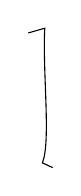
\begin{tikzpicture}[x=1cm,y=1cm]
\draw[line width=.4pt] (2.82,2.96) -- (3.03,3.02) .. controls (3.00,2.48) and (3.11,1.58) .. (3.00,1.31) -- (3.13,1.25);
\end{tikzpicture}}}
\margin{\inserted{\handwritten{\shortstack[l]{\mbox{\begin{tikzpicture}[baseline=0cm,x=1cm,y=1cm]
\draw[line width=.5pt] (0,-.25) -- (.17,.22) .. controls (.20,.39) and (.31,.29) .. (.24,.20) -- (.15,.16);
\end{tikzpicture}} $F$ n'a pas de\\cycles premiers\\immergés \unsure{passant}\\par $x$.}}}}
